\chapter{Сегнетоэлектрические материалы}\label{ch:ch2}
\todo{уже была секция сегнетоэлектрики, подумай над структурой}
\section{Перовскитоподобные материалы/материалы перовскитной структуры}
Классическими материалами, обладающими СЭ свойствами являются перовскитоподобные материалы вида ABO\(_3\), в частности Pb[Zr\(_x\)Ti\(_{1-x}\)]O\(_3\) (PZT) (рис. \cref{fig:pzt})

\begin{figure}[ht]
    \centerfloat{
        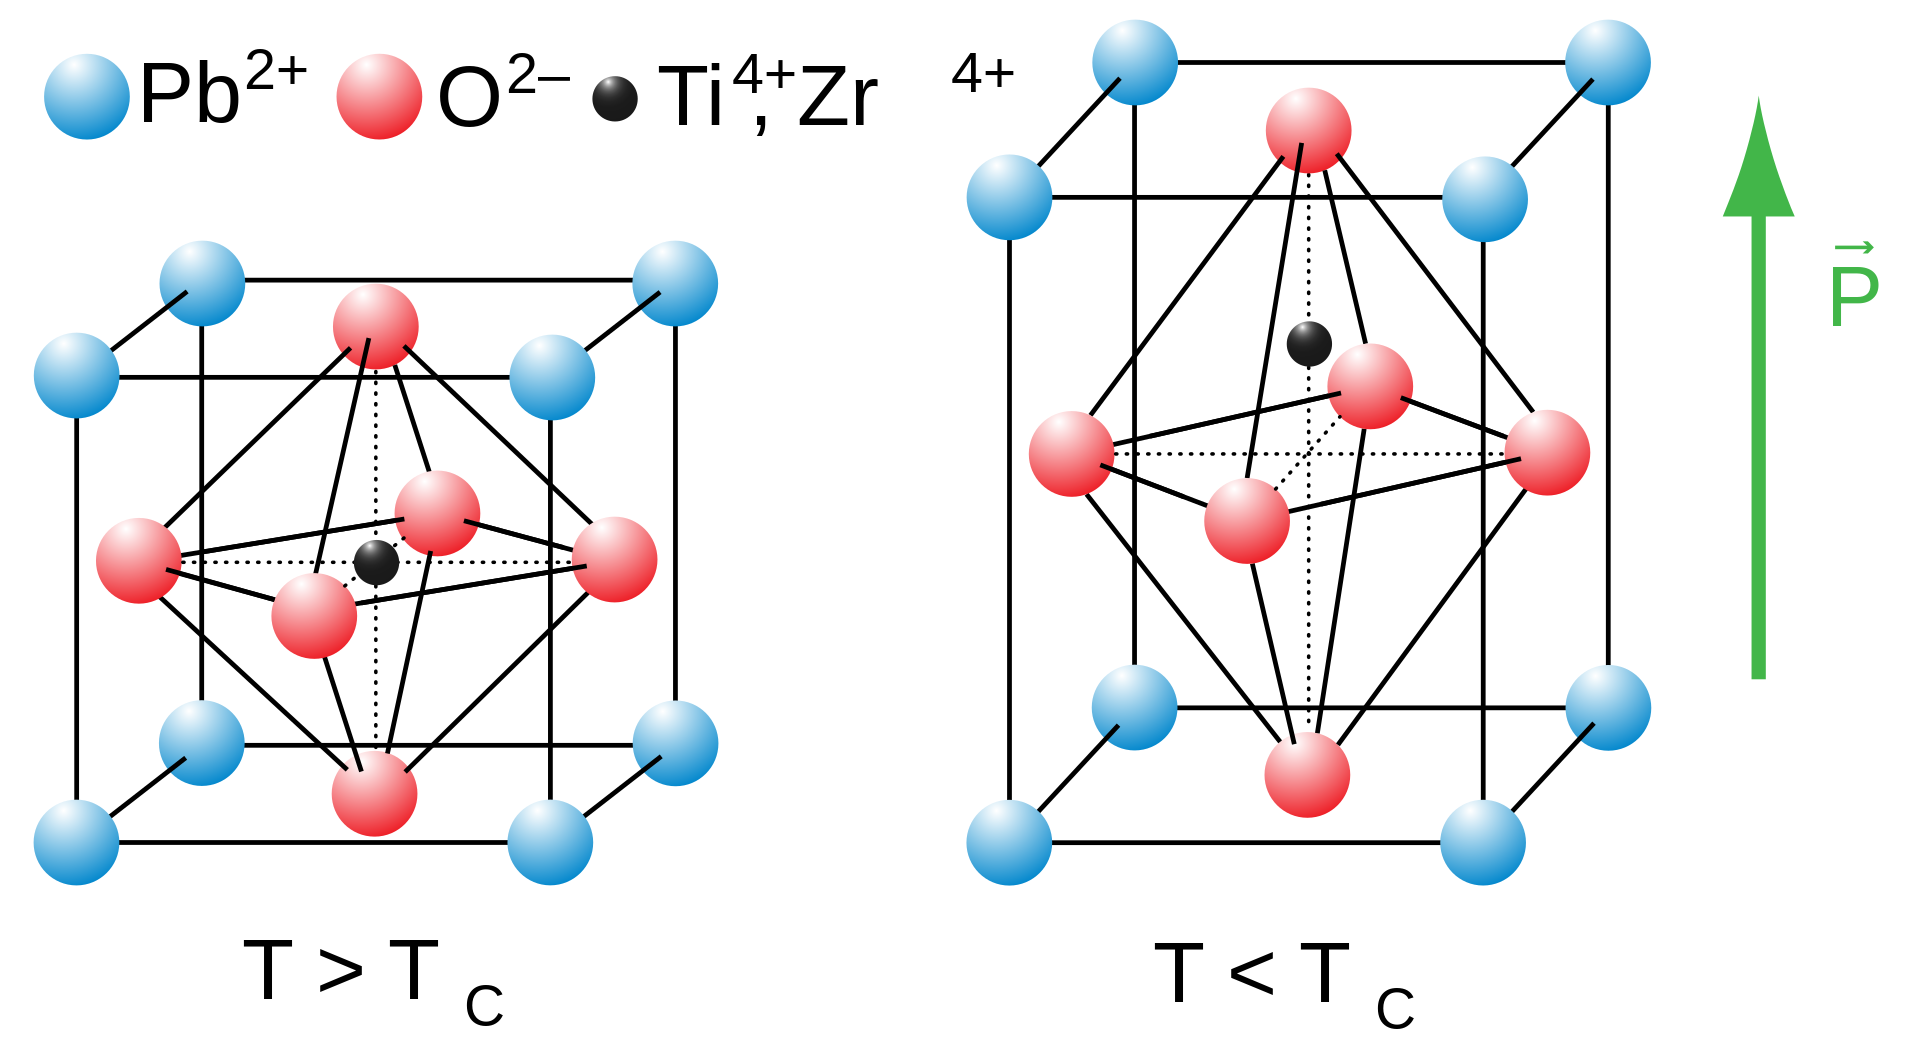
\includegraphics[width=0.8\linewidth]{pzt.png}
    }
    \caption{Кристаллическая структура PZT при температурах выше и ниже точки Кюри \(T_c\)}\label{fig:pzt}
\end{figure}

Необходимость создания слоёв с толщиной сегнетоэлектрического слоя \(~\) \SI{70}{\nano\meter} существенно ограничивает возможность масштабирования устройств на основе перовскитных материалов \cite{parkReviewPerspectiveFerroelectric2018}. Уменьшение толщины приводит к возрастанию тока утечек, что приводит к невозможности достоверного считывания состояния ячейки.
\section{Сегнетоэлектрический оксид гафния}\label{sec:ch2/sec1}
Другим перспективным и интересным для исследования материалом является HfO\(_2\). В 2007 было сообщено об использовании данного материала (наряду с ZrO\(_2\)) в качестве подзатворного диэлектрика в полевом транзисторе для уменьшения токов утечки через подзатворный слой \cite{bohrHighkSolution2007}. В 2011 году в оксиде гафния были обнаружены СЭ свойства \cite{bosckeFerroelectricityHafniumOxide2011}.

При нормальных условиях в оксиде гафния энергетически выгодной является неполярная моноклинная фаза \(P2_1/c\), неполярная орторомбическая \(Pbca\), полярная орторомбическая \(Pca2_1\). Однако, при определённых условиях возможна стабилизация полярной (сегнетоэлектрической) орторомбической фазы \(Pca2_1\). Сегнетоэлектрические свойства при этом определяются отсутствием центральной симметрии в кристаллической решётке.
Было показано, что за снижение свободной энергии сегнетоэлектрической фазы и её стабилизацию в оксиде гафния отвечает ряд характеристик. Так, необходим существенный вклад поверхностной энергии в свободную энергию, который достигается при достаточном уменьшении толщины плёнки. Кроме того, значительным фактором, влияющим на стабилизацию фазы являются механические напряжения в оксиде гафния. Известно, что в отсутствии верхнего электрода сегнетоэлектрические свойства структур на основе оксида гафния значительно ухудшаются. Этот эффект объясняется тем, что при быстрой термической обработке структуры с нижним и верхним электродами, в оксиде гафния возникают механические напряжения, которые образуются за счёт различия в коэффициенте теплового расширения материалов электродов и оксида гафния и приводят к образованию орторомбической фазы за счёт подавления образования моноклинной фазы. Наконец, важнейшим элементом является легирование оксида. Сегнетоэлектрические свойства разной степени выраженности были получены в плёнках с примесями Si \cite{}, Zr \cite{}, La \cite{}, Gd \cite{}, Y \cite{}, Ga \cite{chouprikNanoscaleDopingIts2022}. Несмотря на широкий спектр возможностей по выбору примесного элемента, использование большинства из указанных элементов приводит к повышению температуры кристаллизации плёнки значительно выше 400 \si{\degreeCelsius}, тем самым нарушая возможную совместимость с backend-of-line (BEOL) процессом в CMOS технологии \cite{schmitzLowTemperatureThin2018}, существенно затрудняя внедрение устройств памяти на основе оксида гафния в производство. Одним из наиболее перспективных материалов для создания энергонезависимой памяти является твёрдый раствор Hf0.5Zr0.5O2. Обладая сравнительно невысокой температурой кристаллизации \(\approx\) \SI{400}{\degreeCelsius}, и одинаковой долей элементов Hf и Zr, позволяющей контролировать стехиометрию с большой точностью, HZO ... структуры на основе имеют ... остаточной поляризации (или не надо про это пока)
\section{Моделирование процесса напыления}\label{sec:ch2/sec2}
% Для бла-бла было произведено моделирование
Для моделирования взаимодействия частиц платины с HZO были произведены квантовомеханические расчёты столкновений с помощью пакета SRIM \todo{ref}. Оценка энергии налетаемых частиц была получена с помощью расчёта кинетической энергии атомов при лазерной абляции:
\todo{добавить интуиции к формулке}
\[\bar{E} = 9.92 \cdot 10^{4} A^{1/8} \tau^{1/4} Z^{3/4} (Z+1)^{3/8} (I\lambda)^{1/2}k,\] где \(A\) -- атомная масса распыляемого элемента, \(\tau\) -- длительность импульса, \(Z\) -- средний заряд ионов, вылетающих при абляции, \(I\) -- интенсивность лазерного излучения в \si{\watt}/\si{\cm}\(^2\), \(\lambda\) -- длина волны лазера, \(k\) -- постоянная Больцмана.

При импульсном лазерном напылении использовался лазер Nd:YAG с длиной волны \(\lambda=\) \SI{1064}{\nano\meter}, длительностью импульсов \(\tau=\) \SI{10}{\nano\second}. Интенсивность оценивалась как \(I=\alpha(1-\beta)\frac{J}{S}\), где \(\alpha=(1-R)^{2N}\) -- коэффициент прохождения излучения через \(N=5\) элементов оптической системы, изготовленных из кварцевого стекла с отражательной способностью \(R=0.0337\) \cite{polyanskiyRefractiveindexInfoDatabase2024} для длины волны \(\lambda\) (поглощение при этом не учитывалось), \(\beta=0.748\) -- отражательная способность платины \cite{weberHandbookOpticalMaterials2003}, \(J\) -- энергия одного импульса, \(S\) -- площадь лазерного пятна.
\todo{упомянуть Z из книжки}

\begin{table} [htbp]
    \centering
    \begin{threeparttable}% выравнивание подписи по границам таблицы
        \caption{Название таблицы}\label{tab:Ts0Sib}%
        \begin{tabular}{ | p{2.5cm} | p{3cm} | p{3cm} | p{2.3cm}l | }
            \hline
            \hline
            \centering \(J\), \si{\milli\joule} & \centering \(I\), \si{\giga\watt}/\si{\cm}\(^2\) & \centering \(\bar{E}\), \si{\electronvolt} & \centering \(d\), \si{\nm} & \\
            \hline
            \centering 225                      & \centering  13.4                                 & \centering  151                            & \centering  1.3            & \\
            \centering 145                      & \centering  8.6                                  & \centering  121                            & \centering 1.2             & \\
            \centering 93                       & \centering  5.5                                  & \centering  97                             & \centering 1.1             & \\
            \centering 45                       & \centering  2.7                                  & \centering  68                             & \centering 1.0             & \\
            \hline
            \hline
        \end{tabular}
    \end{threeparttable}
\end{table}

На рисунке \cref{fig:pt_distr} показано \todo{вероятностное} распределение атомов платины в слое HZO при \todo{... многократном} ... Стоит отметить, что при распылении проникновение частиц платины в HZO быстро заканчивается: расстояние между плоскостями (111) в кубической гранецентрированной решётке составляет \(\frac{a}{\sqrt{3}}\approx\) \SI{2.26}{\angstrom}, поэтому структурные свойства HZO могут измениться лишь при напылении \(\sim 4-5\) первых атомных слоёв.

\begin{figure}[ht]
    \centerfloat{
        \hfill
        \subcaptionbox[List-of-Figures entry]{\label{fig:pt_distr_151eV} \SI{151}{\electronvolt}}{%
            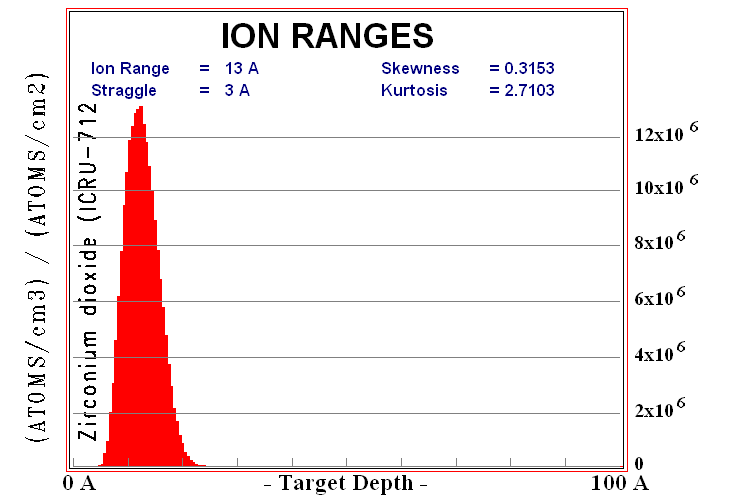
\includegraphics[width=0.5\linewidth]{151 eV.png}}
        \hfill
        \subcaptionbox{\label{fig:pt_distr_121eV}\SI{121}{\electronvolt}}{%
            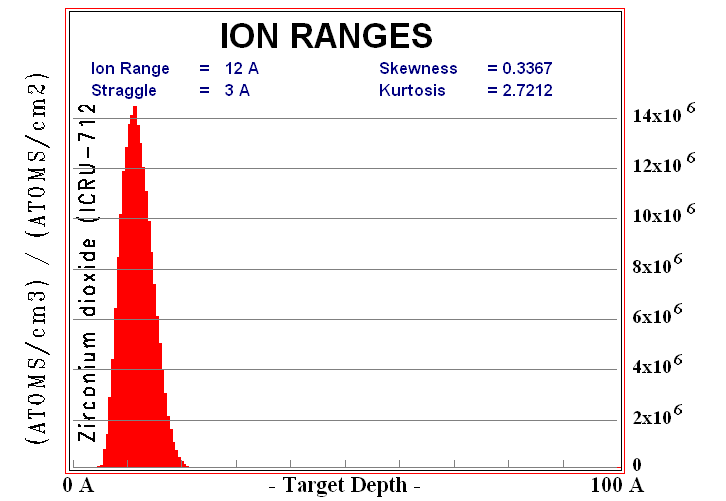
\includegraphics[width=0.5\linewidth]{121 eV.png}}
        \hfill
        \\
        \subcaptionbox{\label{fig:pt_distr_97eV}\SI{97}{\electronvolt}}{%
            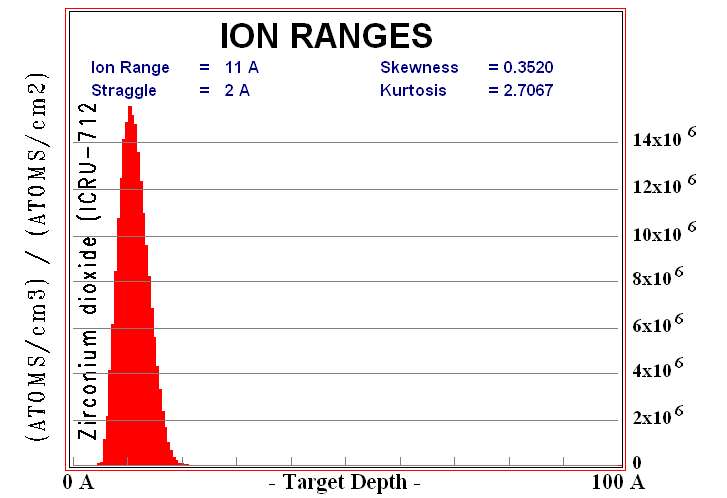
\includegraphics[width=0.5\linewidth]{97 eV.png}}
        \hfill
        \subcaptionbox{\label{fig:pt_distr_68eV}\SI{68}{\electronvolt}}{%
            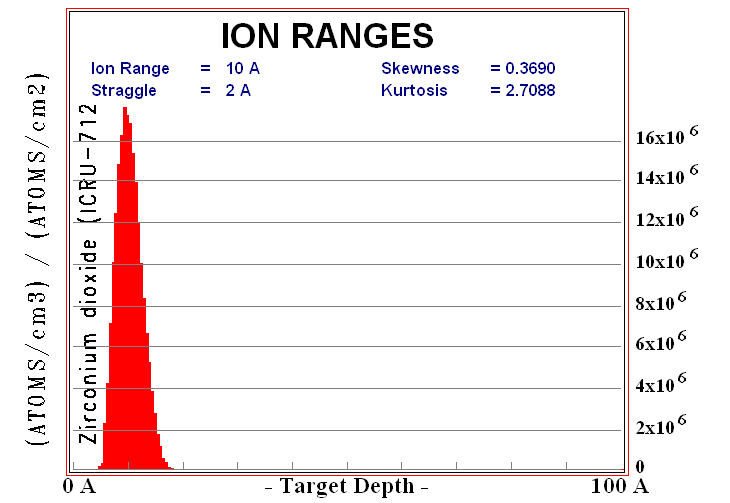
\includegraphics[width=0.5\linewidth]{68 eV.png}}
        \hfill
    }
    \caption[Этот текст попадает в названия рисунков в списке рисунков]{Распределение атомов платины в плёнке HZO \todo{после 100 000 актов распыления} при различных энергиях распыляемых частиц}\label{fig:pt_distr}
\end{figure}

% Одна ссылка: \cite[с.~54]{Sokolov}\cite[с.~36]{Gaidaenko}.
% Две ссылки: \cite{Sokolov,Gaidaenko}.
% Ссылка на собственные работы: \cite{vakbib1, confbib2}.
% Много ссылок: %\cite[с.~54]{Lermontov,Management,Borozda} % такой «фокус»
%вызывает biblatex warning относительно опции sortcites, потому что неясно, к
%какому источнику относится уточнение о страницах, а bibtex об этой проблеме
%даже не предупреждает
% \cite{Lermontov, Management, Borozda, Marketing, Constitution, FamilyCode,
%     Gost.7.0.53, Razumovski, Lagkueva, Pokrovski, Methodology, Berestova,
%     Kriger}%
% \ifnumequal{\value{bibliosel}}{0}{% Примеры для bibtex8
%     \cite{Sirotko, Lukina, Encyclopedia, Nasirova}%
% }{% Примеры для biblatex через движок biber
%     \cite{Sirotko2, Lukina2, Encyclopedia2, Nasirova2}%
% }%
% .
% И~ещё немного ссылок:~\cite{Article,Book,Booklet,Conference,Inbook,Incollection,Manual,Mastersthesis,
%     Misc,Phdthesis,Proceedings,Techreport,Unpublished}
% % Следует обратить внимание, что пробел после запятой внутри \cite{}
% % обрабатывается ожидаемо, а пробел перед запятой, может вызывать проблемы при
% % обработке ссылок.
% \cite{medvedev2006jelektronnye, CEAT:CEAT581, doi:10.1080/01932691.2010.513279, doi:10.1021/acsami.0c16741,
%     Gosele1999161,Li2007StressAnalysis, Shoji199895, test:eisner-sample,
%     test:eisner-sample-shorted, AB_patent_Pomerantz_1968, iofis_patent1960}%
% \ifnumequal{\value{bibliosel}}{0}{% Примеры для bibtex8
% }{% Примеры для biblatex через движок biber
%     \cite{patent2h, patent3h, patent2}%
% }%
% .

\section{Микроскопия пьезоотклика}
Микроскопия пьезоотклика основана на измерении пьезоэлектрического отклика с помощью атомно-силовой микроскопии (АСМ)
\subsection{Атомно-силовая микроскопия}
Atomic Force Microscopy (AFM) is a high-resolution imaging technique that allows the mapping of
atomic-scale features on a material’s surface. It is generally characterized by its ability to provide
three-dimensional topographic images at extremely high spatial resolutions, as high as fractions of
a nanometer, which is much smaller than the wavelength of visible light.
47
Chapter 2: Fabrication and Measurement Techniques
The primary component of AFM is a sharp probe, or tip, at the end of a cantilever, typically made
from silicon or silicon nitride. As this tip is brought very close to the surface, it interacts with the
surface atoms through van der Waals forces or other types of attractive or repulsive forces.
The deflection of the cantilever caused by this tip-surface interaction is measured using a laser
beam, which is reflected from the top of the cantilever into a position-sensitive detector. A feedback
loop is then used to maintain constant force between the tip and the sample, providing an accurate
map of the surface topography.
AFM can operate in multiple modes, including contact mode, tapping mode and hybrid mode, each
with its advantages and suitable applications. Furthermore, it is not only limited to topographical
imaging; many advanced AFM techniques can measure electrical, mechanical, magnetic, and
thermal properties of surfaces at the nanoscale.
One of the key advantages of AFM over other microscopy techniques like electron microscopy is
its ability to image samples in their natural environments, without the need for special sample
preparation like coating or vacuum conditions. This feature makes AFM particularly useful for
biological and chemical research, though its applications extend to physics, materials science,
nanotechnology, and many other fields.
Despite these advantages, AFM does have its limitations, such as slower scan speeds compared to
other methods and difficulties imaging highly rough or tall samples due to the physical constraints
of the cantilever. Nevertheless, AFM remains an essential tool in the exploration of the nanoscale
world

\nomenclature{FEM}{finite element method, метод конечных элементов}
\nomenclature{HZO}{Hf0.5Zr0.5O2, оксид гафния-циркония}
\nomenclature{АСО}{атомно-слоевое осаждение}
\nomenclature{АСМ}{атомно-силовая микроскопия}
\nomenclature{PUND}{positive up negative down, электрофизический метод измерения остаточной поляризации}
\nomenclature{CMOS}{complementary metal-oxide-semiconductor, комплементарная структура металл-оксид-полупроводник}
\nomenclature{БТО}{быстрая термическая обработка}
\nomenclature{NVM}{non-volatile memory, энергонезависимая память}
\nomenclature{FIT}{finite integration technique, метод конечных интегралов}
\nomenclature{FMM}{fast multipole method, быстрый метод многополюсника}
\nomenclature{FVTD}{finite volume time-domain, метод конечных объёмов
    во~временной области}
\nomenclature{MLFMA}{multilevel fast multipole algorithm, многоуровневый
    быстрый алгоритм многополюсника}
\nomenclature{BEM}{boundary element method, метод граничных элементов}
\nomenclature{CST MWS}{Computer Simulation Technology Microwave Studio
    программа для компьютерного моделирования уравнен Максвелла}
\nomenclature{DDA}{discrete dipole approximation, приближение дискретиных
    диполей}

\FloatBarrier
